
%----------------------------------------------------------------------------------------
%	Settings and packages
%----------------------------------------------------------------------------------------

\documentclass[10pt]{article}

\usepackage{colortbl}
\usepackage{multirow}
\usepackage[table]{xcolor}
\usepackage{ctable}
\usepackage{float}
\usepackage[landscape,margin=0.25in,legalpaper]{geometry}

\newcommand{\mcn}[2]{\multicolumn{#1}{l}{#2}}	
\newcommand{\mccn}[2]{\multicolumn{#1}{c}{#2}}
\newcommand{\mcl}[1]{\multicolumn{2}{l}{#1}}
\newcommand{\mclg}[1]{\multicolumn{2}{l}{\gr #1}}
\newcommand{\mcc}[1]{\multicolumn{2}{c}{#1}}
\newcommand{\mccg}[1]{\multicolumn{2}{c}{\gr #1}}
\newcommand{\mr}[1]{\multirow{-2}{*}{#1}}
\definecolor{Gray}{gray}{0.90}
\newcommand{\gr}{\cellcolor{Gray}}

\newcommand{\thickline}{\specialrule{.1em}{.05em}{.05em}}

\setlength\parindent{0pt}

% column colours
\newcolumntype{g}{>{\columncolor{Gray}}l}
\newcolumntype{w}{>{\columncolor{white}}l}

%----------------------------------------------------------------------------------------
%	Table
%----------------------------------------------------------------------------------------

\begin{document}

\thispagestyle{empty}
{\bf 2014 Deepwell Cup}
\begin{table}[h!]
    \centering
    \begin{tabular}{l g g w w g g w w g g w w g g w w g g}
        \rowcolor{black}\mcn{19}{\color{white}\bf Round 3: Conference Finals} \\
        \rowcolor{white}\\
        &  \mccg{Andre D}&  \mcc{Charmaine L}&  \mccg{David D}&  \mcc{Kollin H}&  \mccg{Kyle L}&  \mcc{Mark D}&  \mccg{Michael D}&  \mcc{Nathaniel T}&  \mccg{Thomas L} \\\thickline
        {\bf East} &&&&&&&&&&&&&&&&&&\\\hline
          New York Rangers&&&&&&&&&&&&&&&&&&\\
          Montreal Canadiens & \mr{MTL} & \mr{7} & \mr{NYR} & \mr{7} & \mr{MTL} & \mr{6} & \mr{NYR} & \mr{7} & \mr{MTL} & \mr{6} & \mr{NYR} & \mr{5} & \mr{MTL} & \mr{7} & \mr{MTL} & \mr{6} & \mr{NYR} & \mr{6}\\\hline
          &&&&&&&&&&&&&&&&&& \\
        {\bf West} &&&&&&&&&&&&&&&&&&\\\hline
          Chicago Blackhawks&&&&&&&&&&&&&&&&&&\\
          Los Angeles Kings & \mr{CHI} & \mr{7} & \mr{CHI} & \mr{7} & \mr{CHI} & \mr{7} & \mr{CHI} & \mr{7} & \mr{CHI} & \mr{7} & \mr{CHI} & \mr{7} & \mr{CHI} & \mr{6} & \mr{CHI} & \mr{7} & \mr{CHI} & \mr{6}\\\hline
          \rowcolor{white}\\
        \rowcolor{black} \mcn{19}{\color{white}\bf Conference Champions} \\
          Eastern & \mclg{PIT} & \mcl{BOS} & \mclg{BOS} & \mcl{BOS} & \mclg{BOS} & \mcl{BOS} & \mclg{BOS} & \mcl{MTL} & \mclg{BOS}\\
          Western & \mclg{ANA} & \mcl{ANA} & \mclg{COL} & \mcl{CHI} & \mclg{CHI} & \mcl{SJS} & \mclg{CHI} & \mcl{ANA} & \mclg{ANA}\\
          Stanley Cup & \mclg{PIT} & \mcl{BOS} & \mclg{COL} & \mcl{BOS} & \mclg{BOS} & \mcl{BOS} & \mclg{BOS} & \mcl{MTL} & \mclg{BOS}
    \end{tabular}
\end{table}

{\bf Points}\\
\begin{minipage}{12cm}
    \begin{tabular}{l l}
        Correct team:	& $7$\\
        Correct series length (regardless of series winner):	& $10$\\
        Stanley Cup champion:	& 25\\
        Stanley Cup finalist:	& 15\\
    \end{tabular}

    \vspace{1cm}
    {\bf Number of picks per team:}\\
    \begin{tabular}{lc | lc }
        NYR & 4 & CHI & 9 \\
        MTL & 5 & LAK & 0 \\
    \end{tabular}
\end{minipage}
\begin{minipage}[t]{13cm}
    \begin{figure}[H]
        \vspace{-2.5cm}
        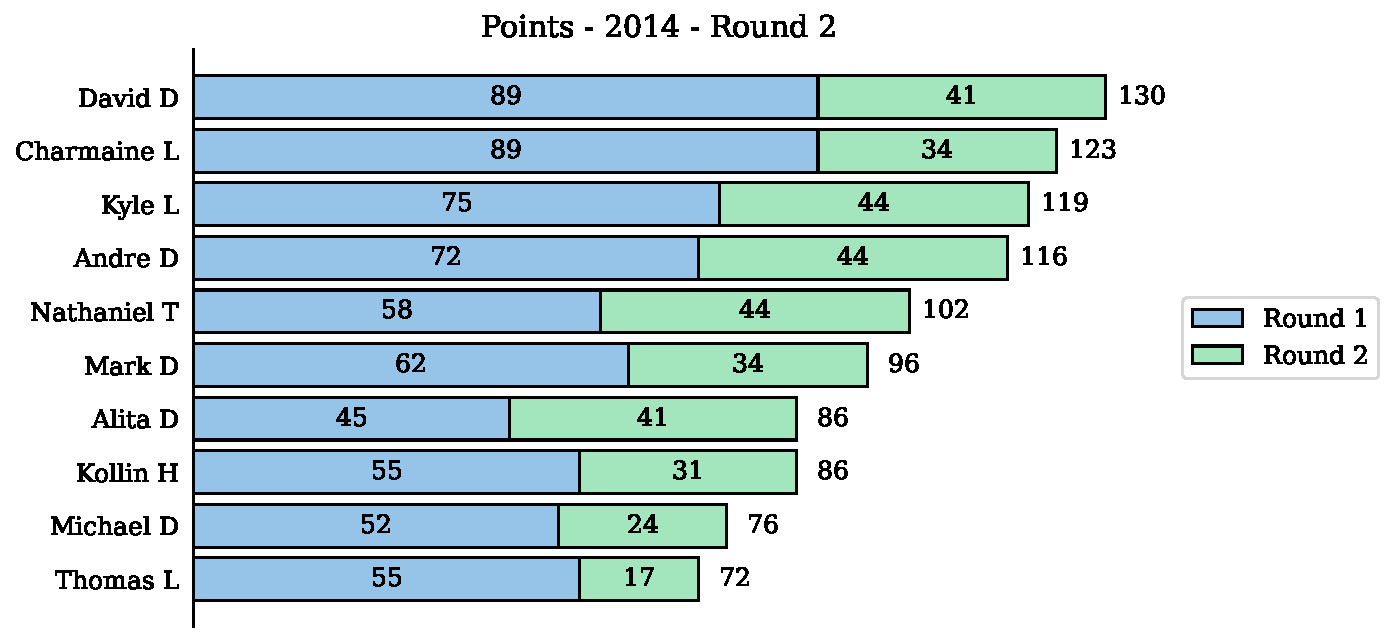
\includegraphics[width=13cm]{../../figures/2014/Points-2014-Round2.pdf}
    \end{figure}
\end{minipage}

\end{document}